\documentclass[11pt]{article}

\usepackage{times}
\usepackage{graphicx}
\usepackage{amsmath}

\textwidth=6.5in
\textheight=8.75in
\oddsidemargin=0.0in
\evensidemargin=0.0in
\topmargin=-0.5in

\begin{document}
\thispagestyle{empty}

\begin{center}
{\bf CS 6300} \hfill {\large\bf HW01:  Search} \hfill {\bf Ryan Dalby} \hfill {\bf Due 25 January 2022}
\end{center}

Please use \LaTeX\ to produce your writeups. See the Homework Assignments 
page on the class website for details.

\section{Uninformed Search}

Consider the state space graph shown below.  A is the start state and
G is the goal state. The costs for each edge are shown on the graph.
Each edge can be traversed in both directions.

\begin{center}
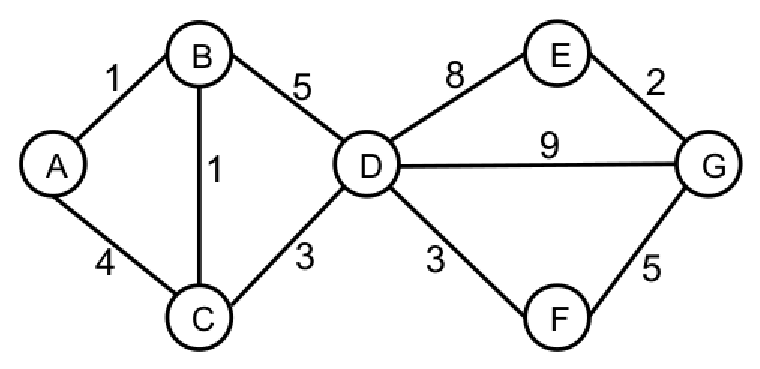
\includegraphics[width=3.5in]{search_graph.eps}
\end{center}

Execute the following search algorithms using priority queues, by
filling in the search table for each part.  (Not all steps will
necessarily be used.)

\vspace{.25in}
Note that for each of the searches below nodes already included in the closed list (previously expanded nodes) were not added to the priority queue.
Also note that alphabetical priority was enforced for tie breaks of depth or cost, where G had highest alphabetical priority.

  \begin{enumerate}

  \item {\bf Breadth First Graph Search.} \\    

    \begin{center}
    \begin{tabular}{|l|l@{\hspace*{1in}}|l|} \hline
    \bf Step & \bf Priority Queue & \bf Expand \\ \hline
    1 & (A,1) & A \\ \hline
    2 & (A-B,2), (A-C,2) & B \\ \hline
    3 & (A-B-C,3), (A-B-D,3), (A-C,2) & C \\ \hline
    4 & (A-B-C,3), (A-B-D,3), (A-C-B,3), (A-C-D,3) & D \\ \hline
    5 & (A-B-D-E,4), (A-B-D-G,4), (A-B-D-F,4), (A-C-B,3), (A-C-D,3) & G \\ \hline
    6 & (A-B-D-G,4) is the solution &  \\ \hline
    \end{tabular}
    \end{center}
  
    Note that for step 4 (A-B-C,3) was not expanded since C was on the closed list, it was subsequently dropped from the priority queue.

    Note that for step 5 (A-C-B,3) and (A-C-D,3) were not expanded since B and D were on the closed list respectively, they were subsequently dropped from the priority queue.

\clearpage

  \item {\bf Depth First Graph Search.} \\

    \begin{center}
    \begin{tabular}{|l|l@{\hspace*{1in}}|l|} \hline
    \bf Step & \bf Priority Queue & \bf Expand \\ \hline
    1 & (A,1) & A \\ \hline
    2 & (A-B,2), (A-C,2) & B \\ \hline
    3 & (A-B-C,3), (A-B-D,3), (A-C,2) & C \\ \hline
    4 & (A-B-C-D,4), (A-B-D,3), (A-C,2) & D \\ \hline
    5 & (A-B-C-D-E,5), (A-B-C-D-G,5), (A-B-C-D-F,5), (A-B-D,3), (A-C,2) & G \\ \hline
    6 & (A-B-C-D-G,5) is the solution &  \\ \hline
    \end{tabular}
    \end{center}

  \item {\bf  Uniform Cost Graph Search.} \\

    \begin{center}
    \begin{tabular}{|l|l@{\hspace*{1in}}|l|} \hline
    \bf Step & \bf Priority Queue & \bf Expand \\ \hline
    1 & (A,0) & A \\ \hline
    2 & (A-B,1), (A-C,4) & B \\ \hline
    3 & (A-B-C,2), (A-B-D,6), (A-C,4) & C \\ \hline
    4 & (A-B-C-D,5), (A-B-D,6), (A-C,4) & D \\ \hline
    5 & (A-B-C-D-E,13), (A-B-C-D-G,14), (A-B-C-D-F,8), (A-B-D,6) & F  \\ \hline
    6 & (A-B-C-D-E,13), (A-B-C-D-G,14), (A-B-C-D-F-G,13) & G \\ \hline
    7 & (A-B-C-D-F-G,13) is the solution &  \\ \hline
    \end{tabular}
    \end{center}

    Note that for step 4 (A-C,4) was not expanded since C was on the closed list, it was subsequently dropped from the priority queue.

    Note that for step 5 (A-B-D,6) was not expanded since D was on the closed list, it was subsequently dropped from the priority queue.

\end{enumerate}

\clearpage

\section{Heuristic Search}

   \begin{enumerate}
  
   \item Consider the two heurisitics $h_1$ and $h_2$, only one of
     which is consistent.  Which one is consistent?

     $h_1$ \textbf{is} consistent because $\quad \forall{X,Y} \quad h_1(X)-h_1(Y) \le cost(X,Y)$ where $X$ and $Y$ are nodes in the state space graph.

     Note that $h_2$ is \textbf{not} consistent, a counter example that violates consistency is $h_1(B)-h_1(C) = 2 > cost(B,C) = 1$.



\begin{center}
\begin{tabular}{|c|c|c|c|c|c|c|c|}\hline
Node  & A   & B  & C  & D  & E   & F   & G  \\ \hline
$h_1$ & 9.5 & 9	 & 8  & 7  & 1.5 & 4   & 0  \\ \hline
$h_2$ & 10  & 12 & 10 & 8  & 1   & 4.5 & 0  \\ \hline
\end{tabular}
\end{center}

  \item Then do A* search with that heuristic.

    \begin{center}
    \begin{tabular}{|l|l@{\hspace*{1in}}|l|} \hline
    \bf Step & \bf Priority Queue & \bf Expand \\ \hline
    1 & (A,9.5) & A \\ \hline
    2 & (A-B,10), (A-C,12) & B \\ \hline
    3 & (A-B-C,10), (A-B-D,13), (A-C,12) & C \\ \hline
    4 & (A-B-C-D,12), (A-B-D,13), (A-C,12) & D \\ \hline
    5 & (A-B-C-D-E,14.5), (A-B-C-D-G,14), (A-B-C-D-F,12), (A-B-D,13) & F \\ \hline
    6 & (A-B-C-D-E,14.5), (A-B-C-D-G,14), (A-B-C-D-F-G,13), (A-B-D,13) &  \\ \hline
    7 & (A-B-C-D-F-G,13) is the solution &  \\ \hline
    \end{tabular}
    \end{center}

    Note that for step 4 (A-C,12) was not expanded since C was on the closed list, it was subsequently dropped from the priority queue.

    Note that for step 6 the tie-break of (A-B-C-D-F-G,13) and (A-B-D,13) went to (A-B-C-D-F-G,13) by tie-break rules before even checking the closed list.

  \item Suppose you are completing the new heuristic function $h_3$
    shown below.  All the values are fixed except $h_3(B)$.

\begin{center}
\begin{tabular}{|c|c|c|c|c|c|c|c|}
\hline
Node & A & B & C & D & E & F & G \\
\hline
$h_3$& 10 & ?  & 9 & 7 & 1.5 & 4.5& 0 \\
\hline
\end{tabular}
\end{center}

For each of the following conditions, write the set of values that are
possible for $h_3(B)$.  For example, to denote all non-negative
numbers, write [0, $\infty$], to denote the empty set, write
$\emptyset$, and so on.

\begin{enumerate}

\item What values of $h_3(B)$ make $h_3$ admissible?

% \[
% \text{If negative heuristic values permitted:} \quad h_3(B) = [-\infty, 12] 
% \]
% \[
% \text{otherwise:} \quad h_3(B) = [0, 12]
% \]
\[
h_3(B) = [0, 12]
\]

\item What values of $h_3(B)$ make $h_3$ consistent?

\[
h_3(B) = [9, 10]
\]

\item What values of $h_3(B)$ will cause A* graph search to expand
  from node A to C, then node A to B, then node A to B to D in that
  order?

\[
h_3(B) = (12, 13)
\]

\end{enumerate}

\end{enumerate}

\end{document}
